\chapter[Metodología del estado del arte]{Metodología del estado del arte}{Metodología del estado del arte}\label{appen3}
\renewcommand{\tablename}{Tabla}


\section{Metodología SLR}

La revisión sistemática de literatura (SLR) es un método que nos permite interpretar y sintetizar de forma adecuada la información obtenida de un tema de investigación. Dado que se ejecuta una manera sistemática sus ventajas son un incremento en la posibilidad de tener mejores resultados en la búsqueda de información \parencite{kitchenhamSystematicLiteratureReviews2009}. Hay tres fases principales en una SLR: (1) Planificación de revisión, (2) Realización de la revisión, (3) Reporte de resultados.

\paragraph{Planificación de revisión}

Esta fase se centra en: (1) La identificación de la necesidad de realizar el SLR, (2) formular las preguntas de investigación que guían la ejecución del SLR, (3) generar la búsqueda de cadenas, y (4) la selección de las fuentes de información para la extracción de los estudios primarios.

\paragraph{Realización de la revisión}

La segunda fase del SLR corresponde a la definición de los criterios de inclusión y exclusión, la ejecución de un proceso de selección de estudios y la evaluación de la calidad de los mismos, lo que da lugar a la selección de los estudios primarios.\\

La metodología se aplicará a tres factores clave de la tesis: el pronóstico del precio, análisis de métricas de la blockchain y la clasificación de precios de la criptomoneda. 


\section{Pronóstico del precio del bitcoin}

\subsection{Planificación de revisión}
\subsubsection{Identificar la necesidad de realizar el SLR}
Tener un enfoque sistemático a la hora de comparar y escoger un algoritmo para la predicción del bitcoin es crucial por la cantidad de datos e información que se pueden obtener hoy día con actualización constante. Una buena comprensión de las variables explicativas, formateo de datos y métodos para comparar los modelos es fundamental a la hora de comprender el modelo propuesto.

\subsubsection{Definiendo las preguntas de investigación}
Las preguntas de investigación para este estudio son las siguientes:

\begin{itemize}
	\item ¿Cuál es el estado del arte de modelos estadísticos para pronósticos del bitcoin?
	\item ¿Cómo implementar trading con bitcoin?
	\item ¿Cuales son los modelos de pronósticos más utilizados?
	\item ¿Qué modelos de aprendizaje máquina se están utilizando?
	\item ¿Cuál es el mejor modelo para realizar pronóstico del bitcoin?
\end{itemize}

\subsubsection{Generar las cadenas de búsqueda}
Para facilitar la búsqueda de los estudios primarios se identificaron las palabras clave resultantes de las preguntas de investigación. Resultaron en las siguientes:

\begin{itemize}
	\item Bitcoin
	\item Machine learning
	\item Trading
	\item Forecasting
\end{itemize}

Combinando las palabras clave con el uso de conectores lógicos “AND” y “OR”, la siguiente cadena de búsqueda es obtenida:\\

\centerline{Bitcoin \textbf{AND} (machine learning \textbf{OR} trading \textbf{OR} forecasting)}

\subsubsection{Selección de fuentes de información}
Las siguientes fuentes de información fueron seleccionadas para la extracción de los estudios:
\begin{itemize}
	\item Google Scholar
	\item IEEE Xplorer
	\item ELSEVIER Science
	\item Springer Link
\end{itemize}

\subsection{Realización de la revisión}
\subsubsection{Criterio de inclusión y exclusión}
Para filtrar los estudios no relevantes para esta investigación se definen los criterios de inclusión y exclusión, que da lugar a los presentados en la \autoref{tab:Table1}.

\begin{table}[h!]
	\centering
	\begin{tabular}{ | m{7cm}| m{7cm} | }
		\hline
		\textbf{Criterio de inclusión} & \textbf{Criterio de exclusión}\\
		\hline
		
		Los primeros estudios mas relevantes según los filtros de búsqueda de las fuentes de información seleccionadas.& Estudios no relevantes según los filtros de búsqueda de las fuentes de información.\\
		
		\hline
		El título contiene la palabra clave ``Bitcoin'' y al menos otra palabra clave. &  El título no contiene ninguna palabra clave\\ 
		\hline
		Abstract está relacionado con predicción de precios del bitcoin usando machine learning o métodos estadísticos. & Estudios que no están relacionados con la predicción del
		bitcoin.\\
		\hline
		Estudios que contienen enfoques de metodologías, modelos, métodos, técnicas de predicción del bitcoin. & Estudios relacionados con el bitcoin pero no tienen un
		enfoque en ciencia de datos.\\
		\hline
		Estudios que contengan resultados sobre la predicción del precio del bitcoin con sus respectivos indicadores de error y comparación con otros métodos. & Estudios con resultados sobre la predicción del bitcoin pero sin comparación de modelos.\\
		\hline
		Estudios publicados entre 2016 y 2020. & Estudios publicados antes del 2016.\\
		\hline
	\end{tabular}
	\caption{Criterios de inclusión y exclusión}
	\label{tab:Table1}
\end{table}

\subsubsection{Selección de estudios primarios}
El protocolo SLR \parencite{kitchenhamSystematicLiteratureReviews2009} sugiere definir un proceso de selección de estudios para obtener los estudios primarios, estructurado de la siguiente manera: (1) aplicar y adaptar la cadena de búsqueda a cada fuente de datos, (2) filtrar los estudios aplicando los primeros criterios de inclusión a cada fuente de información, (3) aplicar el resto de los criterios de inclusión y exclusión, y (4) seleccionar los estudios primarios. Después de aplicar los criterios de inclusión y exclusión como parte del proceso de selección de estudios, se seleccionaron 8 estudios primarios para esta investigación como se ve en la \autoref{fig1}.\\

\begin{figure}[!h]
	\centering
	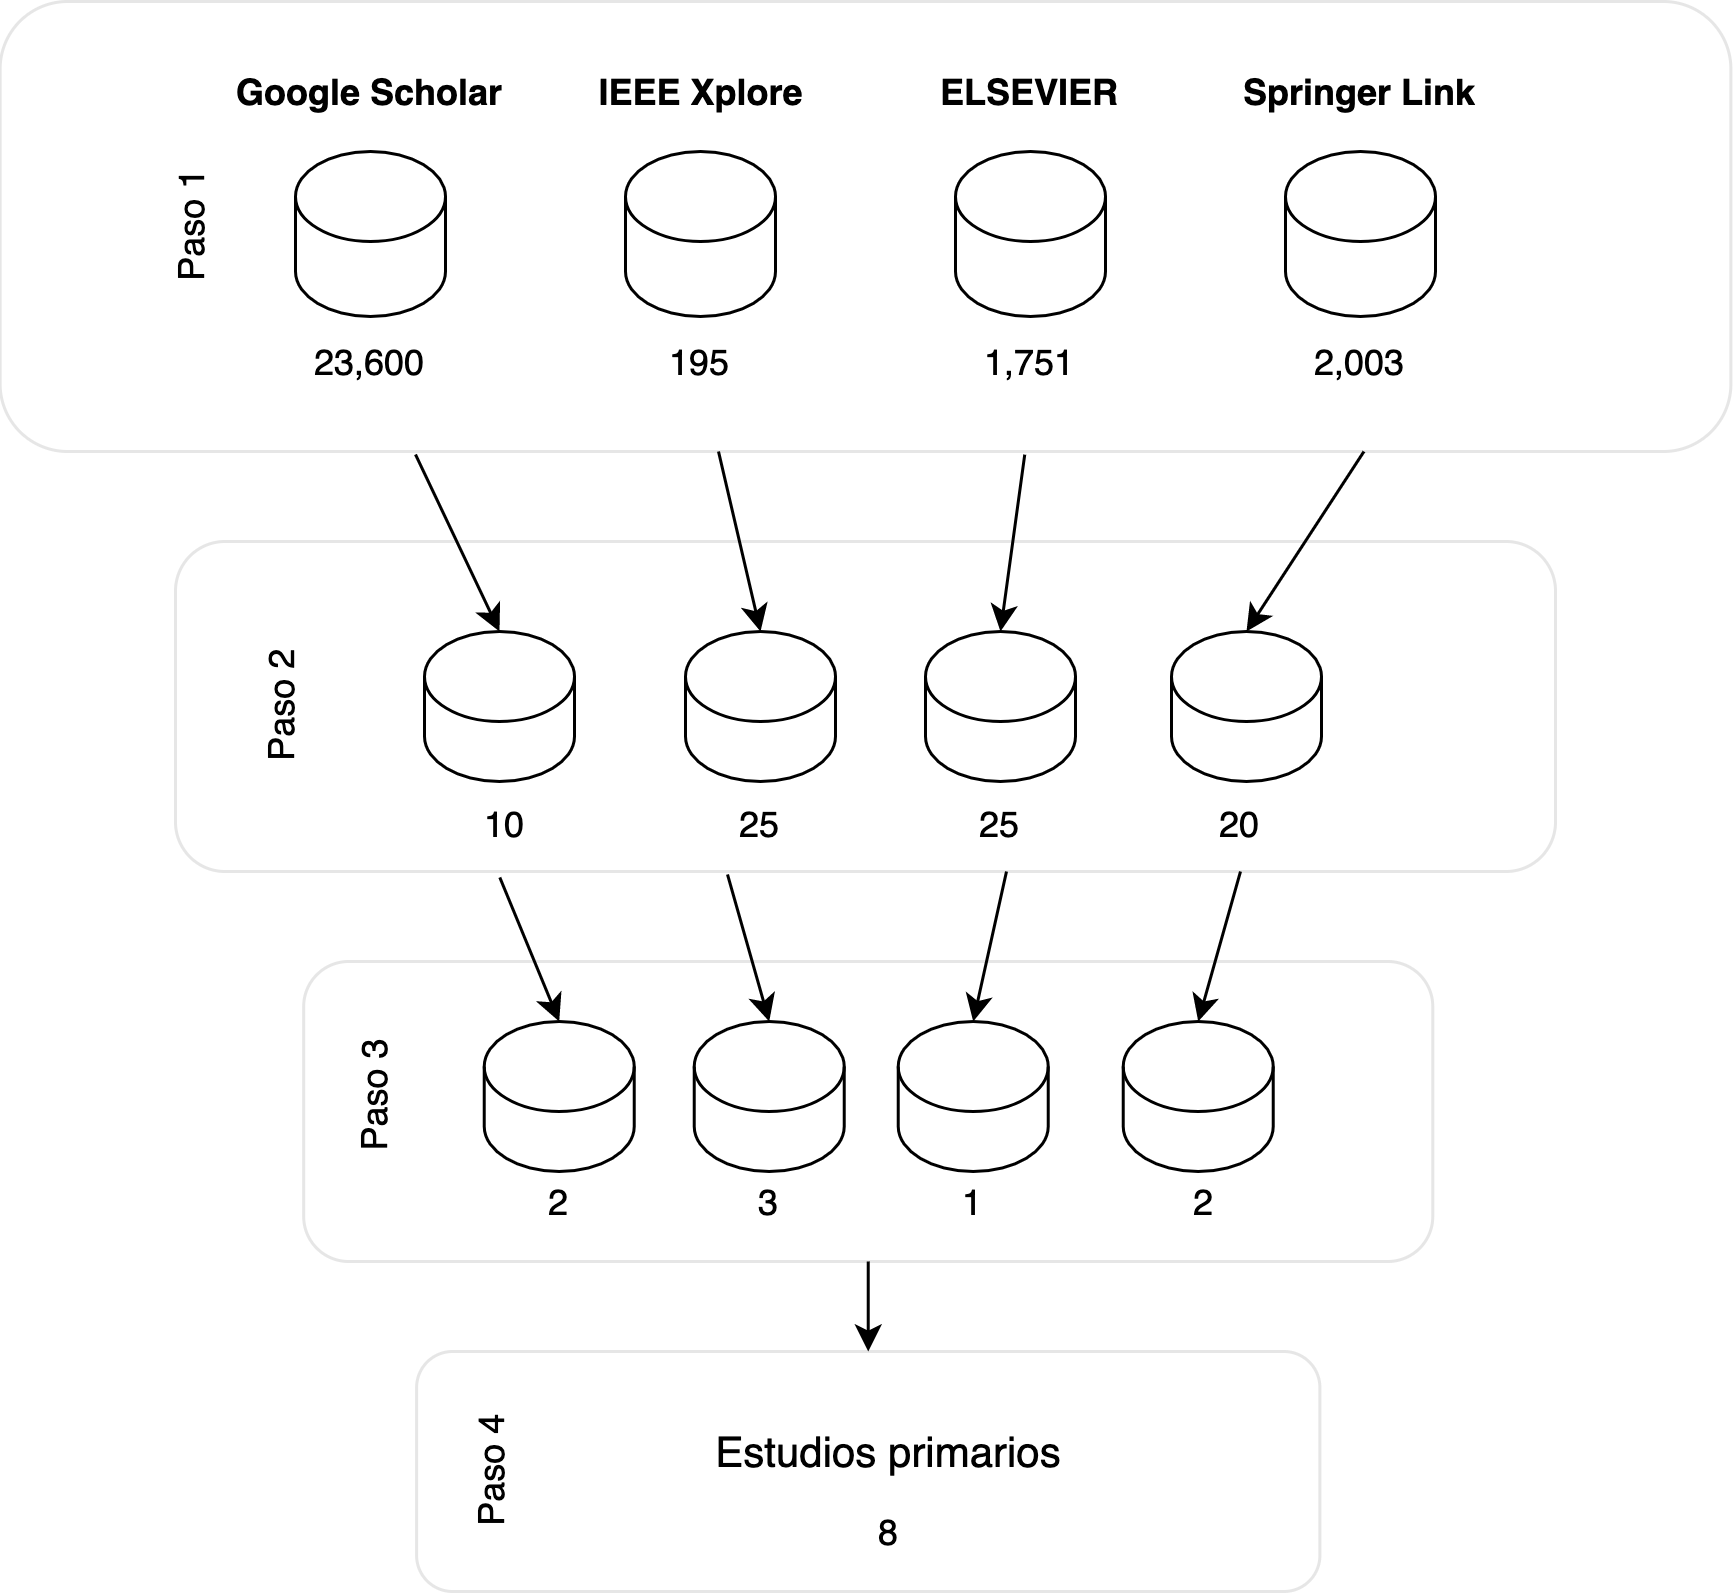
\includegraphics[width=0.7\linewidth]{Chapter2/SelecEstudiPrim_1.png}
	\caption{Selección de estudios primarios y resultados}
	\label{fig1}
\end{figure}

\vspace{-0.5cm}

\subsubsection{Evaluación de la calidad del estudio}
Al evaluar la calidad del estudio, se garantiza que la información contenida en cada uno de los estudios primarios sea pertinente y valiosa para la investigación. En la \autoref{tab:Table2} se presenta la evaluación de la calidad de los estudios que se aplicarán.

\begin{table}[!h]
	\centering
	\begin{tabular}{ | m{2cm}| m{12cm} | }
		\hline
		\textbf{ID} & \textbf{Evaluación de la calidad del estudio}\\
		\hline
		PC1 & ¿El estudio cuenta con una base teórica que explique los métodos utilizados?\\
		\hline
		PC2 & ¿El estudio detalla el método con el cuál pronostica y que variables explicativas utiliza para hacer la predicción?\\
		\hline
		PC3 & ¿El estudio compara modelos de predicción para pronosticar el precio del bitcoin?\\
		\hline
		PC4 & ¿El estudio utiliza algoritmos de machine learning para realizar la predicción?\\
		\hline
		PC5 & ¿El estudio muestra un modelo con mejor rendimiento comparado con los demás?\\
		\hline
	\end{tabular}
	\caption{Evaluación de la calidad del estudio}
	\label{tab:Table2}
\end{table}

Después de evaluar los estudios primarios utilizando las evaluaciones de calidad antes mencionadas quedaron \textbf{6 estudios primarios} \parencite{tandonBitcoinPriceForecasting2019,chenBitcoinPricePrediction2020,mudassirTimeseriesForecastingBitcoin2020,felizardoComparativeStudyBitcoin2019,mcnallyPredictingPriceBitcoin2018,phaladisailoedMachineLearningModels2018}.

\section{Análisis de métricas de la blockchain}
\subsection{Planificación de revisión}
\subsubsection{Identificar la necesidad de realizar el SLR}

Tener un enfoque sistemático de las métricas que más influyen en el precio del bitcoin es crucial por la cantidad de datos e información que se pueden obtener hoy día con actualización constante, más tratándose de un campo tecnológico con evolución persistente.
Una buena comprensión de las variables explicativas ayuda a mejorar y ahorrar esfuerzos en el entendimiento del asenso y descenso del precio de esta criptomoneda.

\subsubsection{Definiendo las preguntas de investigación}
Las preguntas de investigación son las siguientes:
\begin{itemize}
	\item ¿Con qué métodos se están seleccionando las mejores métricas de la blockchain para predicción del precio?
	\item Actualmente, ¿cuales son las métricas de la blockchain que más influyen en el precio del bitcoin?
	\item ¿Cuánto mejora la predicción con las métricas de la blockchain?
\end{itemize}

\subsubsection{Generar las cadenas de búsqueda}
Para facilitar la búsqueda de los estudios primarios se identificaron las palabras clave resultantes de las preguntas de investigación. Resultaron en las siguientes:
\begin{itemize}
	\item Bitcoin
	\item Blockchain
	\item Metrics
	\item Prediction
	\item Features
\end{itemize}
Combinando las palabras clave con el uso de conectores lógicos “AND” y “OR”, la siguiente cadena de búsqueda es obtenida:\\

\centerline{(Bitcoin \textbf{AND} blockchain \textbf{AND} metrics \textbf{AND} prediction)} 
\centerline{\textbf{OR} (Bitcoin \textbf{AND} features \textbf{AND} prediction)}

\subsubsection{Selección de fuentes de información}
Las siguientes fuentes de información fueron seleccionadas para la extracción de los estudios:\\
\vspace{-1cm}
\begin{itemize}
	\item IEEE Xplore
	\item ELSEVIER Science Direct
	\item Springer Link\\
\end{itemize}
\vspace{-1.5cm}
\subsection{Realización de la revisión}
\subsubsection{Criterio de inclusión y exclusión}
Para filtrar los estudios no relevantes para esta investigación se definen los criterios de inclusión y exclusión, que da lugar a los presentados en la \autoref{tab:Table3}.\\

\begin{table}[h!]
	\centering
	\begin{tabular}{ | m{7cm}| m{7cm} | }
		\hline
		\textbf{Criterio de inclusión} & \textbf{Criterio de exclusión}\\
		\hline
		Los primeros estudios más relevantes según los filtros de búsqueda de las fuentes de información seleccionadas.& Estudios no relevantes según los filtros de búsqueda de las fuentes de información.\\
		\hline
		El titulo contiene la palabra Bitcoin o Blockchain y al menos otra palabra clave.&  El titulo no contiene ninguna palabra clave.\\ 
		\hline
		El estudio muestra el o los método utilizados para la selección de métricas.& El estudio no muestra el o los métodos utilizados para la selección de métricas.\\
		\hline
		Estudios publicados entre 2017-2021&Estudios publicados antes del 2017.\\
		\hline
	\end{tabular}
	\caption{Criterios de inclusión y exclusión}
	\label{tab:Table3}
\end{table}

\begin{figure}[H]
	\centering
	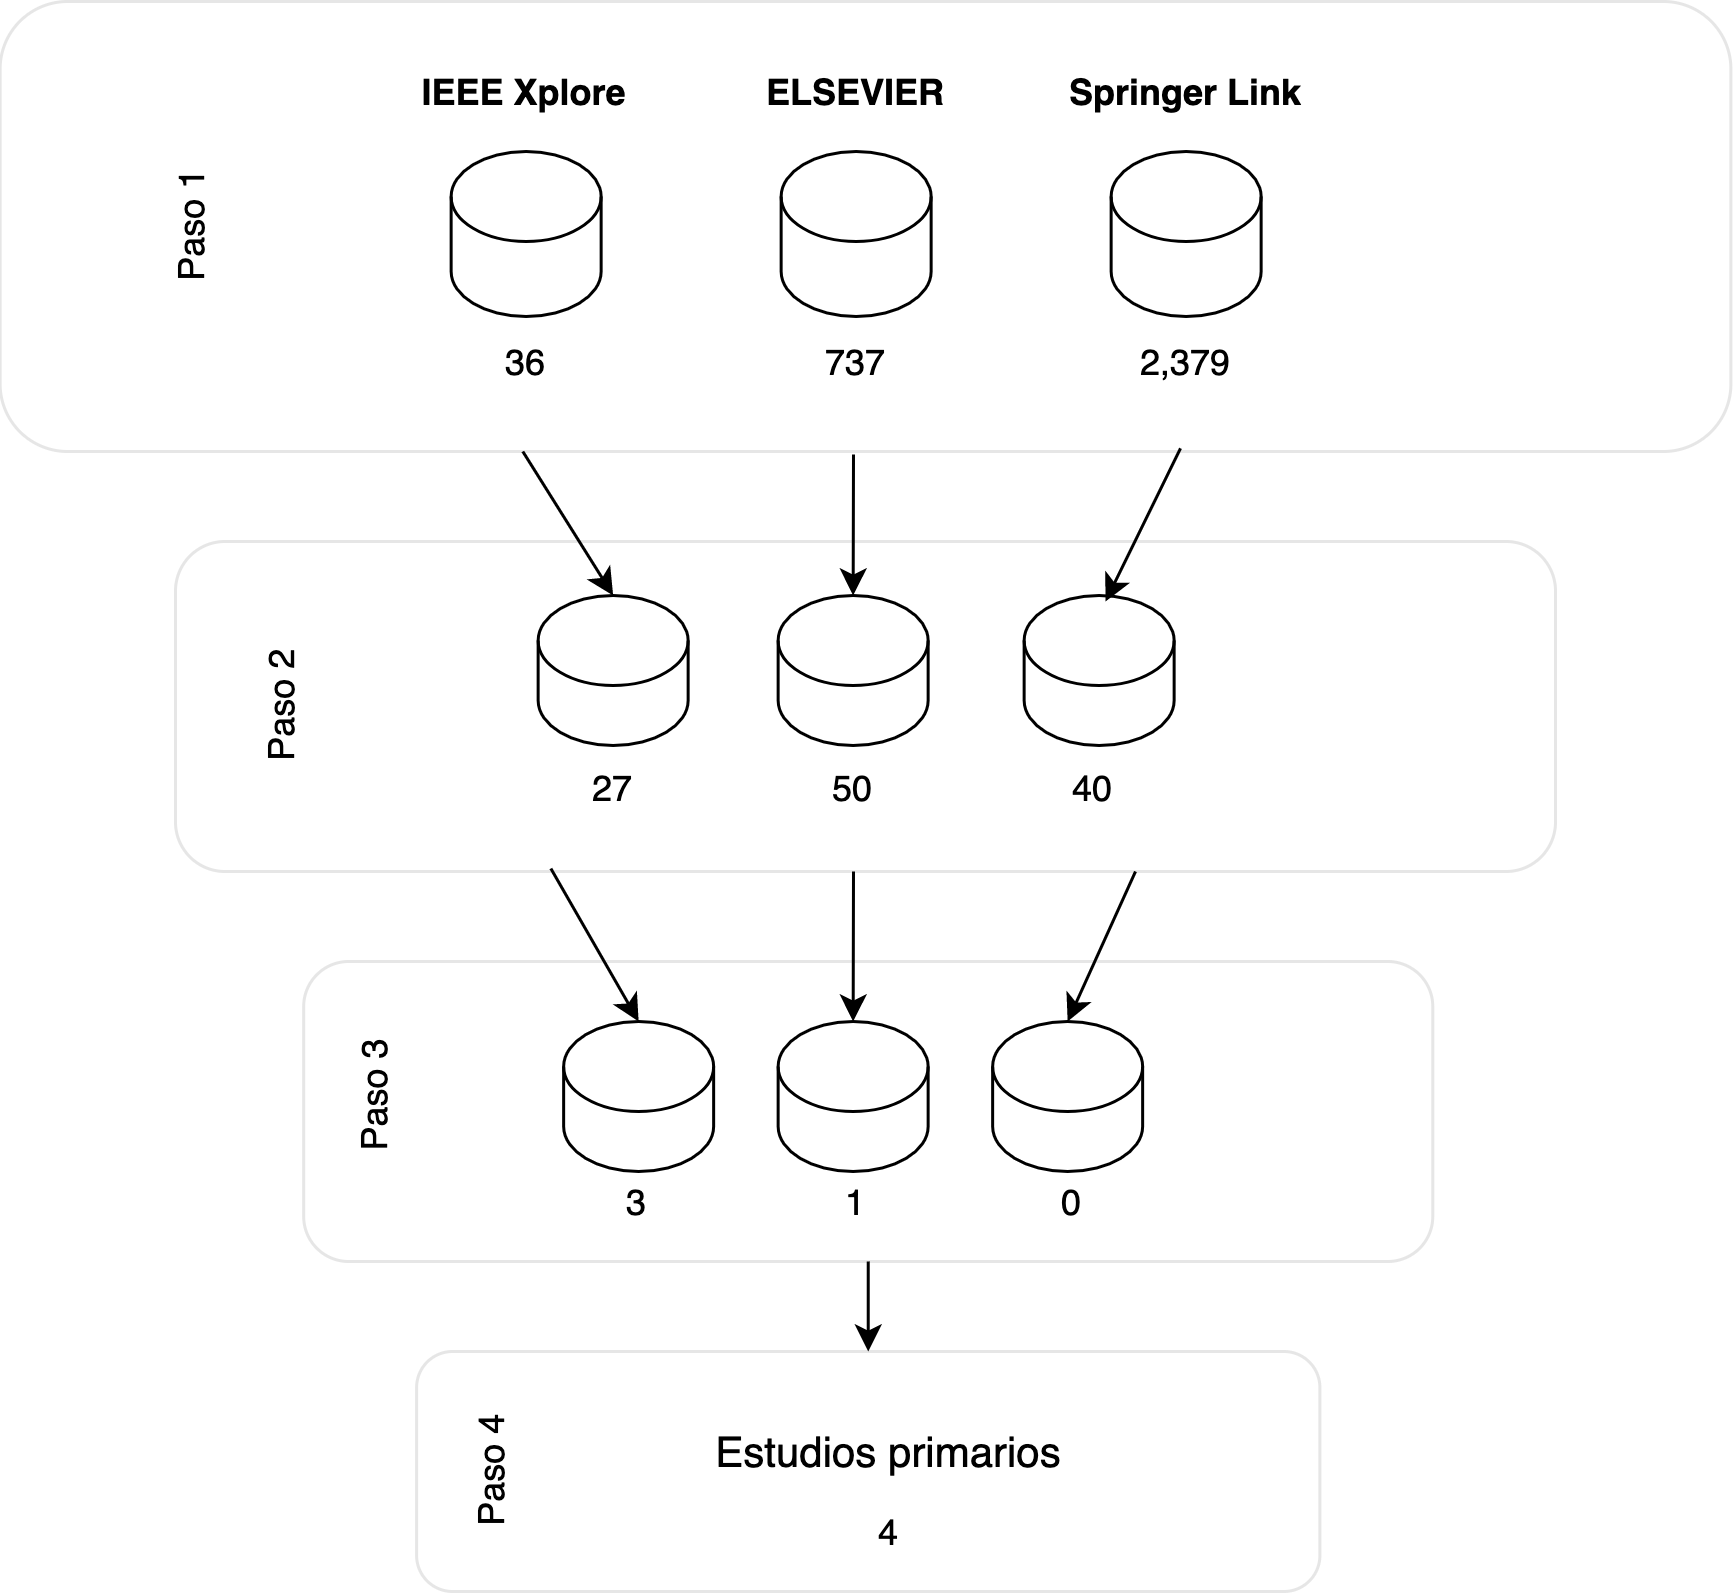
\includegraphics[width=0.7\textwidth]{Chapter2/SelecEstudiPrim_2.png}
	\caption{Selección de estudios primarios y resultados}
	\label{fig2}
\end{figure}
\vspace{-0.8cm}
\subsubsection{Selección de estudios primarios}
Después de aplicar los criterios de inclusión y exclusión como parte del proceso de selección de estudios, se seleccionaron 4 estudios primarios para esta investigación como se ve en la \autoref{fig2}.\\
\vspace{-1cm}
\subsubsection{Evaluación de la calidad del estudio}
Al evaluar la calidad del estudio, se garantiza que la información contenida en cada uno de los estudios primarios sea pertinente y valiosa para la investigación. En la \autoref{tab:Table5} se presenta la evaluación de la calidad de los estudios que se aplicarán.

\begin{table}[H]
	\centering
	\begin{tabular}{ | m{2cm}| m{12cm} | }
		\hline
		\textbf{ID} & \textbf{Evaluación de la calidad del estudio}\\
		\hline
		PC1 & ¿El estudio detalla y explica la metodología utilizada para encontrar las variables explicativas que mejoran la predicción?\\
		\hline
		PC2 & ¿El estudio concluye si agregar variables de la blockchain mejora o no la predicción del bitcoin?\\
		\hline
	\end{tabular}
	\caption{Evaluación de la calidad del estudio}
	\label{tab:Table5}
\end{table}

Después de evaluar los estudios primarios utilizando las evaluaciones de calidad antes mencionadas quedaron 3 estudios primarios \parencite{chenMachineLearningModel2021,jiBestFeatureSelection2019,saadCharacterizingBlockchainbasedCryptocurrencies2018}.

\section{Clasificación del precio para inversión}

\subsection{Planificación de revisión}
\subsubsection{Identificar la necesidad de realizar el SLR}

Un enfoque sistemático de los métodos de clasificación más utilizados es de suma importancia ya que por la existencia de una gran variedad de métodos y cambios constantes en los mismos con un ritmo acelerado pude ser abrumador, por lo anterior el entendimiento de los modelos de clasificación con un enfoque SLR puede impulsar la creación de nuevos modelos más robustos y con mejor precisión.\\

\subsubsection{Definiendo las preguntas de investigación}
Las preguntas de investigación para este estudio son las siguientes:
\begin{itemize}
	\item ¿Qué modelos de clasificación se están utilizando?
	\item ¿Cómo se clasifican los precios del bitcoin para la toma de decisiones de inversión?
	\item ¿Cuál es la mejor metodología para clasificación de precios del bitcoin?
\end{itemize}

\subsubsection{Generar las cadenas de búsqueda}
Para facilitar la búsqueda de los estudios primarios se identificaron las palabras clave resultantes de las preguntas de investigación. Resultaron en las siguientes:
\begin{itemize}
	\item Bitcoin
	\item Blockchain
	\item Investment
	\item Classification
	\item Deep Learning
\end{itemize}
Combinando las palabras clave con el uso de conectores lógicos “AND” y “OR”, la siguiente cadena de búsqueda es obtenida:\\

\centerline{(Bitcoin \textbf{AND} classification \textbf{AND} deep learning)} 
\centerline{\textbf{OR} (Bitcoin \textbf{AND} classification \textbf{AND} deep learning \textbf{AND} investment)}

\subsubsection{Selección de fuentes de información}
Las siguientes fuentes de información fueron seleccionadas para la extracción de los estudios:\\
\begin{itemize}
	\item IEEE Xplore
	\item ELSEVIER Science Direct
	\item Springer Link\\
\end{itemize}
\subsection{Realización de la revisión}
\subsubsection{Criterio de inclusión y exclusión}
Para filtrar los estudios no relevantes para esta investigación se definen los criterios de inclusión y exclusión, que da lugar a los presentados en la \autoref{tab:Table6}.\\

\begin{table}[h!]
	\centering
	\begin{tabular}{ | m{7cm}| m{7cm} | }
		\hline
		\textbf{Criterio de inclusión} & \textbf{Criterio de exclusión}\\
		\hline
		Los primeros estudios más relevantes según los filtros de búsqueda de las fuentes de información seleccionadas.& Estudios no relevantes según los filtros de búsqueda de las fuentes de información.\\
		\hline
		El titulo contiene la palabra Bitcoin o Blockchain y al menos otra palabra clave.&  El titulo no contiene ninguna palabra clave.\\ 
		\hline
		El abstract está relacionado con la clasificación del precios del Bitcoin.& Estudios que no estaban relacionados con la clasificación del precio del bitcoin.\\
		\hline
		Estudios que contienen resultados sobre la clasificación de precios del Bitcoin con sus respectivos indicadores de precisión.& Estudios que no muestran indicadores de precisión de la clasificación.\\
		\hline
		Estudios publicados entre 2017-2021&Estudios publicados antes del 2017.\\
		\hline
	\end{tabular}
	\caption{Criterios de inclusión y exclusión}
	\label{tab:Table6}
\end{table}

\begin{figure}[h!]
	\centering
	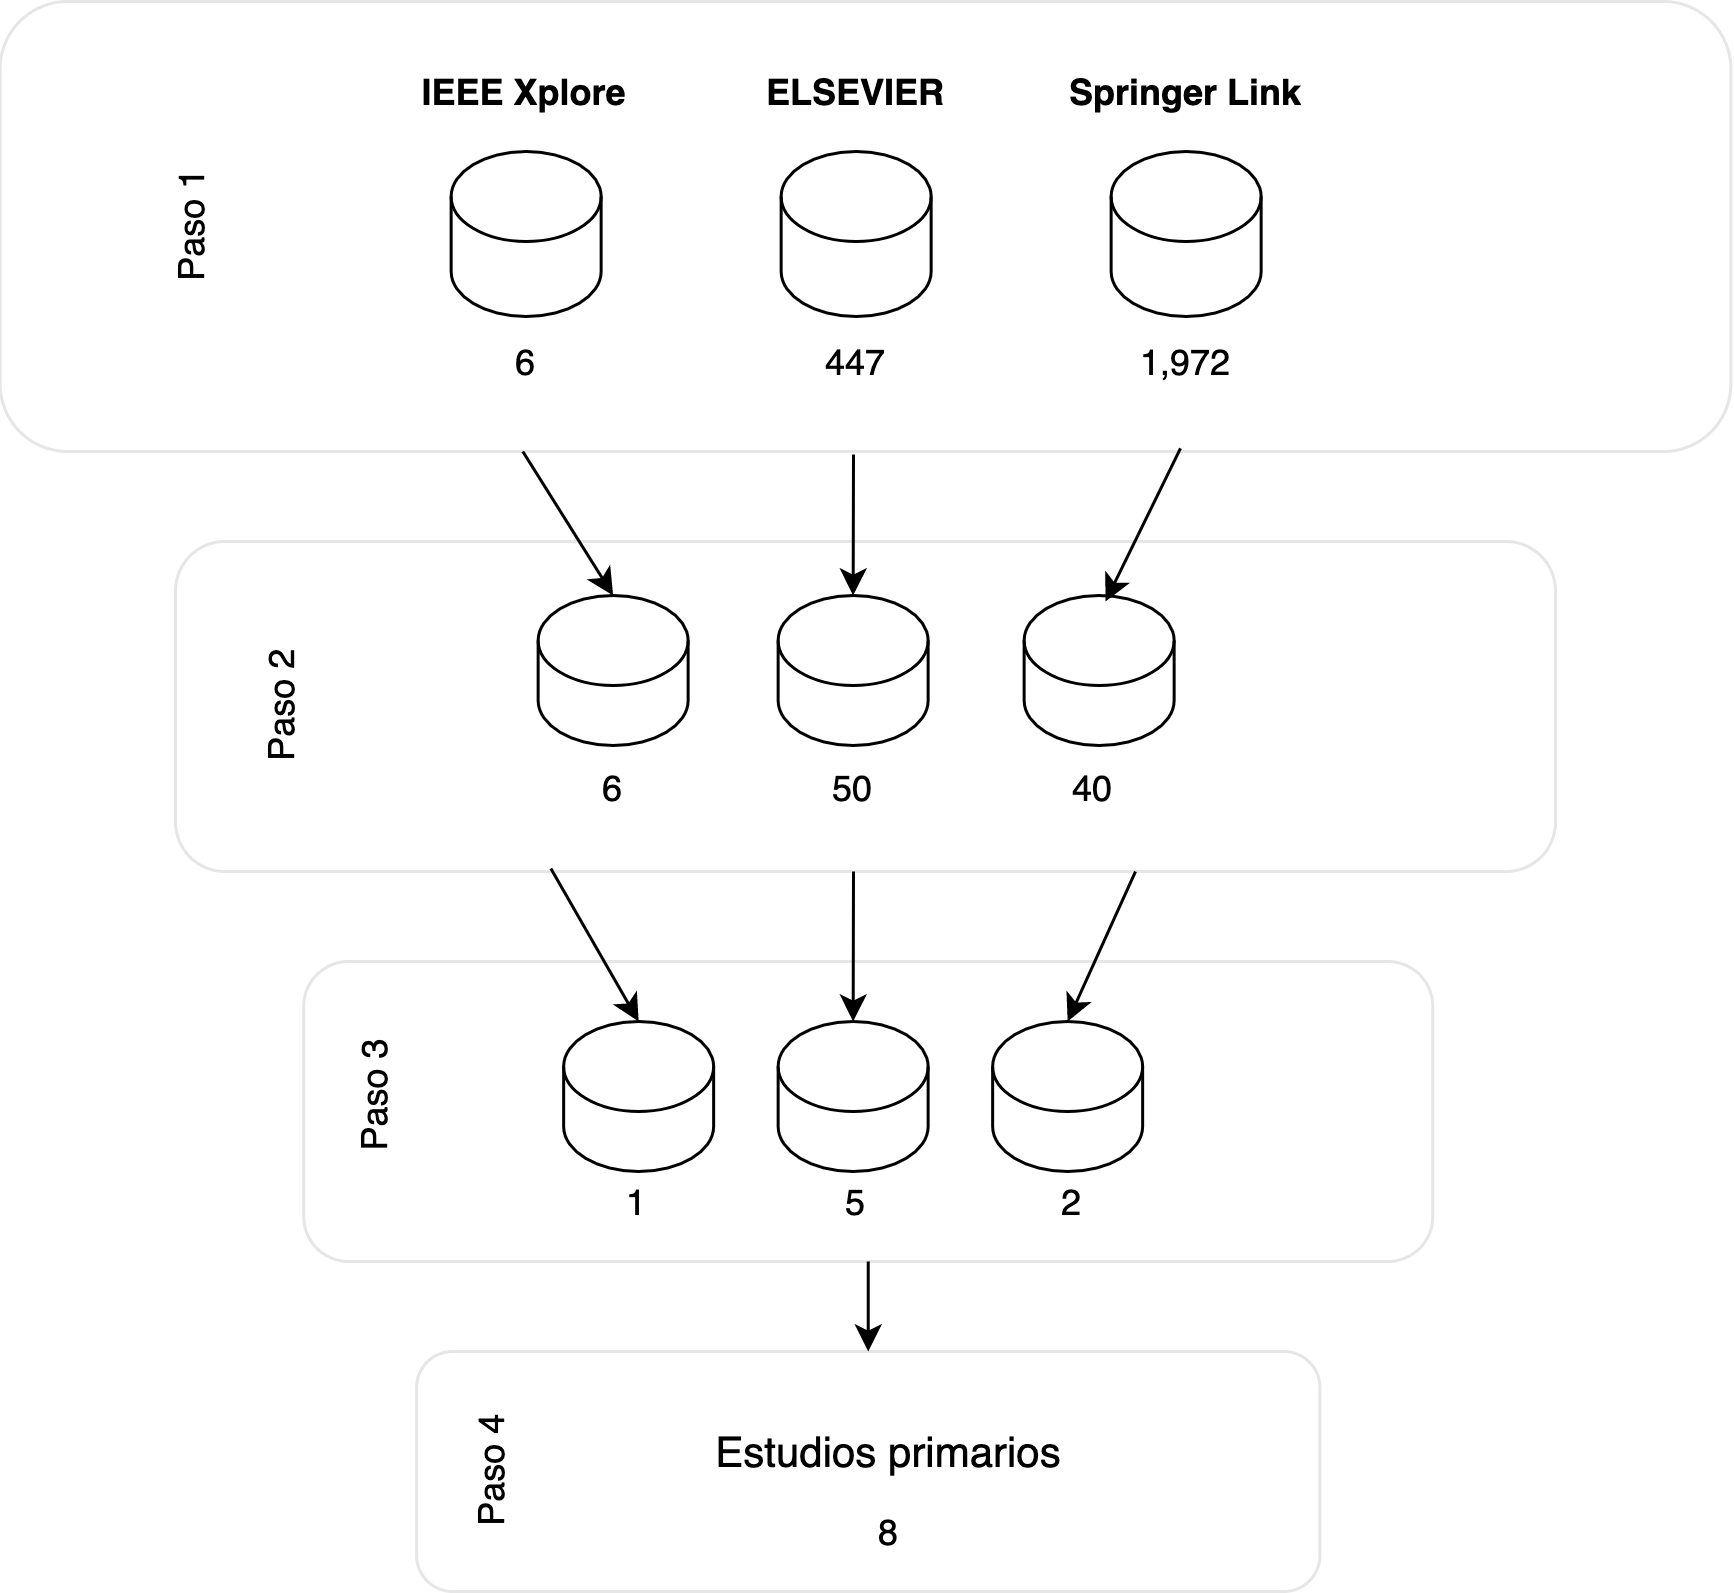
\includegraphics[width=0.7\textwidth]{Chapter2/SelecEstudiPrim_3.png}
	\caption{Selección de estudios primarios y resultados}
	\label{fig3}
\end{figure}

\subsubsection{Selección de estudios primarios}
Después de aplicar los criterios de inclusión y exclusión como parte del proceso de selección de estudios, se seleccionaron 8 estudios primarios para esta investigación como se ve en la \autoref{fig3}.\\

\subsubsection{Evaluación de la calidad del estudio}
Al evaluar la calidad del estudio, se garantiza que la información contenida en cada uno de los estudios primarios sea pertinente y valiosa para la investigación. En la \autoref{tab:Table7} se presenta la evaluación de la calidad de los estudios que se aplicarán.

\begin{table}[H]
	\centering
	\begin{tabular}{ | m{2cm}| m{12cm} | }
		\hline
		\textbf{ID} & \textbf{Evaluación de la calidad del estudio}\\
		\hline
		PC1 & ¿El estudio detalla la metodología utilizada para realizar la clasificación de los precios?\\
		\hline
		PC2 & ¿El estudio da una descripción de los modelos utilizados para realizar la clasificación?\\
		\hline
		PC3 & ¿El estudio muestra un modelo de clasificación con un mejor rendimiento comparado con los demás?\\
		\hline
	\end{tabular}
	\caption{Evaluación de la calidad del estudio}
	\label{tab:Table7}
\end{table}

Después de evaluar los estudios primarios utilizando las evaluaciones de calidad antes mencionadas quedaron 5 estudios primarios \parencite{ibrahimPredictingMarketMovement2021,jaquartShorttermBitcoinMarket2021,chenBitcoinPricePrediction2020,akyildirimPredictionCryptocurrencyReturns2021,pintelasInvestigatingProblemCryptocurrency2020}.

\section{Discusión de la metodología SLR}
En esta sección daremos respuesta a nuestras preguntas de investigación con base en los artículos primarios.

\subsection{Pronóstico del precio del bitcoin}

\textbf{\textit{1.- ¿Cuál es el estado del arte de modelos estadísticos para pronósticos de bitcoin?}}\\
Bitcoin es una criptomoneda altamente usada hoy día, por ello hay algunos modelos para la predicción de su precio, ya sea con modelos estadísticos más tradicionales como regresión lineal o métodos de deep learning como LSTM \parencite{tandonBitcoinPriceForecasting2019}. Sin embargo, algunos inversores no tratan al bitcoin como una moneda de acuerdo al criterio usado por los economistas y hacen una inversión especulativa \parencite{chenBitcoinPricePrediction2020}. Una pregunta natural sería que características tomar en cuenta a la hora de hacer la predicción. Ya que bitcoin no cuenta una tendencia clara y tienen una alta volatilidad entonces los métodos de deep learning son una solución efectiva \parencite{tandonBitcoinPriceForecasting2019}. Más aun, se puede demostrar que es una serie de tiempo no estacionaria \parencite{mudassirTimeseriesForecastingBitcoin2020} y por consiguiente mas conveniente los métodos de aprendizaje maquina, aunque, igualmente, dado que los datos financieros están en el formato OHLCV se muestra que todas las variables están altamente correlacionadas entre si y los métodos estadísticos mas tradicionales pueden ser efectivos \parencite{phaladisailoedMachineLearningModels2018}.\\

\textbf{\textit{2. ¿Cómo implementar trading con bitcoin?}}\\
Hay muchos enfoques a la hora de realizar la compra y venta de este activo, una cantidad numerosa de estudios han llegado a la conclusión de que usando indicadores técnicos del bitcoin se puede predecir con precisión los retornos generados \parencite{mudassirTimeseriesForecastingBitcoin2020}.\\
Por otro lado se tienen estudios que indican que una manera de hacer trading es calcular el cambio del precio en intervalos de una hora \parencite{phaladisailoedMachineLearningModels2018}, al final del día o cada treinta o noventa día basándose en el volumen del movimientos de los precios del bitcoin \parencite{mudassirTimeseriesForecastingBitcoin2020}. También se ha concluido que hacer trading tomando en cuenta las variables asociadas al precio como la apertura, valor máximo, mínimo y cierre, dan buenos resultado \parencite{felizardoComparativeStudyBitcoin2019,phaladisailoedMachineLearningModels2018}. Por ultimo se puede hacer ingeniería de características y tomar características de alta dimensionalidad para realizar trading en intervalos de cinco minutos \parencite{chenBitcoinPricePrediction2020} .\\

\textbf{\textit{3. ¿Cuáles son los modelos de pronósticos más utilizados?}}\\
Dada la naturaleza del precio del bitcoin los métodos de aprendizaje profundo son los favoritos en este caso RNN (Recurrent Neural Network) y LSTM \parencite{mcnallyPredictingPriceBitcoin2018}.\\

\textbf{\textit{4. ¿Qué modelos de aprendizaje máquina se estan utilizando?}}\\
En los estudios comparativos es frecuente utilizar los siguientes modelos: ARIMA, RTS, RF, SVM y LSTM \parencite{felizardoComparativeStudyBitcoin2019,phaladisailoedMachineLearningModels2018}.\\

\textbf{\textit{5. ¿Cuál es el mejor modelo para realizar pronóstico del bitcoin?}}

En la mitad de los estudios primarios seleccionados \parencite{mudassirTimeseriesForecastingBitcoin2020,chenBitcoinPricePrediction2020,mcnallyPredictingPriceBitcoin2018} el mejor modelo de predicción son las redes LSTM basados en la exactitud (accuracy) con una puntuación que va desde un 52.78\% \parencite{mcnallyPredictingPriceBitcoin2018}, hasta un 67.2\% \parencite{chenBitcoinPricePrediction2020}. En los demás estudios se tiene incertidumbre y especifican mas investigación.

\subsection{Análisis de métricas de la blockchain}

\textbf{\textit{1. ¿Con que métodos se están seleccionando las mejores métricas de la blockchain para predicción del precio?}}\\
En la literatura disponible se están utilizando diversas aproximaciones para la selección de métricas con mayor influencia. En los estudios primarios los métodos de correlación \parencite{jiBestFeatureSelection2019,saadCharacterizingBlockchainbasedCryptocurrencies2018} fueron los mas predominantes. En estos se calcula la correlación que existe entre el precio y las características de la blockchain, se seleccionan las que tienen el coeficiente más alto y a su vez mejoran los modelos de predicción que no incluyen las métricas propuestas.
Cambien existen métodos que utilizan análisis de sensibilidad y arboles aleatorios para reducir el subconjunto de predictores midiendo la importancia del factor tecnológico \parencite{chenMachineLearningModel2021}. En este se seleccionaron las métricas con el índice de importancia más alto.\\

\textbf{\textit{2. Actualmente, ¿cuales son las métricas de la blockchain que más influyen en el precio del bitcoin?}}\\
En \parencite{jiBestFeatureSelection2019} se encontró que entre 84 métricas obtenidas las mejores fueron aquellas relacionas con el indice de transacciones nVout que cuenta con cinco variables.
Por otro lado en \parencite{saadCharacterizingBlockchainbasedCryptocurrencies2018} utilizando igualmente análisis de correlación se obtuvo que las métricas con mayor influencia fueron las relacionadas con el número de carteras, la dificultad de minado, el hash rate y UTX's que es el conjunto de salidas de transacciones no gastadas.
Por último en \parencite{chenMachineLearningModel2021} las mejores características de la blockchain fueron la capitalización del mercado, el valor promedio de transacciones, la tasa promedio de transacciones, la dificultad de minado y el tamaño del bloque.\\

\textbf{\textit{3. ¿Cuánto mejora la predicción con las métricas de la blockchain?}}\\
En \parencite{saadCharacterizingBlockchainbasedCryptocurrencies2018,chenMachineLearningModel2021} se utilizo el modelo LSTM para la comparación en las mejoras, en \parencite{chenMachineLearningModel2021} se logró una reducción de hasta 73 dólares en términos del RMSE promedio, mientras que en el error medio absoluto (MAE) se logro una reducción de 606,69 hasta 548,15. Por otro lado en \parencite{saadCharacterizingBlockchainbasedCryptocurrencies2018} se alcanzó un MAE mínimo 0,0889 sobre el conjunto de validación.
En \parencite{jiBestFeatureSelection2019} se utilizo regresión lineal sobre series de tiempo y se alcanzo una precisión del 95,04\%, mostrando una mejora en comparación del estado del arte \parencite{mcnallyPredictingPriceBitcoin2018} donde se logró una precisión del 52,78 \%.

\subsection{Clasificación del precio para inversión}

\textbf{\textit{1. ¿Que modelos de clasificación se están utilizando?}}\\
El estados del arte de los estudios primarios nos muestran que los modelos de machine learning y deep learning son los más populares entre ellos destacando Random Forest (RF), Linear Regresion (LR), Support Machine Vector (SVM), XGBoost y Long short-term memory (LSTM) \parencite{ibrahimPredictingMarketMovement2021, jaquartShorttermBitcoinMarket2021,chenBitcoinPricePrediction2020,akyildirimPredictionCryptocurrencyReturns2021,pintelasInvestigatingProblemCryptocurrency2020}.\\

\textbf{\textit{2. ¿Cómo se clasifican los precios del bitcoin para la toma de decisiones de inversión?}}\\
En la mayoría de estudios la clasificación se realiza para trading, esto es, se clasifica el precio con base en si este sube o baja tomando en cuenta alguna característica que involucre pequeños periodos de tiempo. Se puede encontrar clasificación de precios que toman en cuenta si el precio incrementó en periodos de tiempo de 5, 15, 30, 60 minutos o diariamente \parencite{ibrahimPredictingMarketMovement2021, jaquartShorttermBitcoinMarket2021,chenBitcoinPricePrediction2020,pintelasInvestigatingProblemCryptocurrency2020}. También hay criterios que toman en cuenta si el precio de apertura del día es mayor o menor que el precio de cierre para realizar la clasificación \parencite{akyildirimPredictionCryptocurrencyReturns2021}.\\

\textbf{\textit{3. ¿Cuál es la mejor metodología para clasificación del precio del bitcoin?}}\\
De todos los estudios primarios estudiados el modelo que mejor precisión alcanzó fue LSTM alcanzando un 67,2\% de \textit{accuracy} sobre un intervalo de actualización de 5 minutos \parencite{chenBitcoinPricePrediction2020}. El método propuesto en este estudio se caracteriza por incluir características de alta dimensionalidad como métricas de la blockchain y del mercado.\\






